\documentclass[12pt,oneside]{uhthesis}
\usepackage{subfigure}
\usepackage[ruled,lined,linesnumbered,titlenumbered,algochapter,spanish,onelanguage]{algorithm2e}
\usepackage{amsmath}
\usepackage{amssymb}
\usepackage{amsbsy}
\usepackage{caption,booktabs}
\captionsetup{ justification = centering }
%\usepackage{mathpazo}
\usepackage{float}
\setlength{\marginparwidth}{2cm}
\usepackage{todonotes}
\usepackage{listings}
\usepackage{xcolor}
\usepackage{multicol}
\usepackage{graphicx}
\floatstyle{plaintop}
\restylefloat{table}
\addbibresource{Bibliography.bib}
% \setlength{\parskip}{\baselineskip}%
\renewcommand{\tablename}{Tabla}
\renewcommand{\listalgorithmcfname}{Índice de Algoritmos}
%\dontprintsemicolon
\SetAlgoNoEnd

\definecolor{codegreen}{rgb}{0,0.6,0}
\definecolor{codegray}{rgb}{0.5,0.5,0.5}
\definecolor{codepurple}{rgb}{0.58,0,0.82}
\definecolor{backcolour}{rgb}{0.95,0.95,0.92}

\lstdefinestyle{mystyle}{
    backgroundcolor=\color{backcolour},   
    commentstyle=\color{codegreen},
    keywordstyle=\color{purple},
    numberstyle=\tiny\color{codegray},
    stringstyle=\color{codepurple},
    basicstyle=\ttfamily\footnotesize,
    breakatwhitespace=false,         
    breaklines=true,                 
    captionpos=b,                    
    keepspaces=true,                 
    numbers=left,                    
    numbersep=5pt,                  
    showspaces=false,                
    showstringspaces=false,
    showtabs=false,                  
    tabsize=4
}

\lstset{style=mystyle}

\title{Título de la tesis}
\author{\\\vspace{0.25cm}Nombre del autor}
\advisor{\\\vspace{0.25cm}Nombre del primer tutor\\\vspace{0.2cm}Nombre del segundo tutor}
\degree{Licenciado en (Matemática o Ciencia de la Computación)}
\faculty{Facultad de Matemática y Computación}
\date{Fecha\\\vspace{0.25cm}\href{https://github.com/username/repo}{github.com/username/repo}}
\logo{Graphics/uhlogo}
\makenomenclature

\renewcommand{\vec}[1]{\boldsymbol{#1}}
\newcommand{\diff}[1]{\ensuremath{\mathrm{d}#1}}
\newcommand{\me}[1]{\mathrm{e}^{#1}}
\newcommand{\pf}{\mathfrak{p}}
\newcommand{\qf}{\mathfrak{q}}
%\newcommand{\kf}{\mathfrak{k}}
\newcommand{\kt}{\mathtt{k}}
\newcommand{\mf}{\mathfrak{m}}
\newcommand{\hf}{\mathfrak{h}}
\newcommand{\fac}{\mathrm{fac}}
\newcommand{\maxx}[1]{\max\left\{ #1 \right\} }
\newcommand{\minn}[1]{\min\left\{ #1 \right\} }
\newcommand{\lldpcf}{1.25}
\newcommand{\nnorm}[1]{\left\lvert #1 \right\rvert }
\renewcommand{\lstlistingname}{Ejemplo de código}
\renewcommand{\lstlistlistingname}{Ejemplos de código}

\begin{document}

\frontmatter
\maketitle

\begin{dedication}
    A mis estrellas de luz infinita. 
\end{dedication}

\begin{acknowledgements}
Es irracional pensar que los méritos son virtud exclusiva de quien los obtiene. He tenido la dicha de contar con personas de cariño inagotable que me han formado y enseñado a identificar el camino; o mejor dicho:  ``mi'' camino; cuando apenas veía más que neblina. Me han guiado para convertirme en un buen profesional, pero sobre todas las cosas a ser un buen ser humano porque toda cualidad es poca si la humanidad es escasa. Por enseñarme a ser una persona de familia: a mis estrellas... y a mis estrellas. 

A mis abuelos: a mí abuela Mimi caudal de nobleza y gentileza, siempre con una sonrisa puesta, siempre presente para cada uno de sus nietos. A mi abuela Arminda, servicial como ninguna, amor humanizado.

A mis padres: a mi Mamá con su cariño constante, ejemplo de mujer indestructible, gracias. A mí papá, por enseñarme a conquistar las cosas creo preciadas; porque esperar por regalías es solo síntoma de falta de cordura.

A mis tíos y tías: a Richeld, uno de los hombres más grandes que conozco. A Reinaldo ejemplo de orden e inteligencia. A Agustín inesperadamente espontáneo. A Teresa por sus poemas. A mí tía Mileidy porque no existe mujer más preocupada. A mí tía Perla, la más alegre. A mí tía Yasnay, mujer integral. A mí tía abuela Maria Elena que siempre tiene un tema interesante que debatir. Y a esa tía Ivón que cuida de los míos.

A mis primas: A Thalía que es una suerte de cometa Halley, a Yaimita que persigue sus sueños, a Karla con nuestra eterna disputa, a Flavita, alegría de la casa. Y a Lizette matanzera irremediable.

A los amigos que he tenido, esos compañeros de viaje, que por fortuna no han sido pocos y que de mencionarlos junto a los elogios que les tengo reservados, tomaría más de las 60 páginas que tiene este trabajo. A los profesores que me han instruido y a los tutores de esta tesis por el tiempo.

\:

\:

A mi familia nuevamente, y sin siquiera dudarlo: al hombre mas grande que he conocido y una eterna bailarina. A las castañuelas y a las soldaduras. Gracias.
\end{acknowledgements}
\begin{opinion}
El trabajo ``Lógica para un Gestor de Certificados Académicos'' desarrollado por el estudiante José Alejandro Labourdette - Lartigue Soto, cumple con los requisitos para la culminación de la carrera de Ciencia de la Computación de la Universidad de La Habana.

El trabajo forma parte de una solución descentralizada para un sistema de certificación de títulos académicos basado en la tecnología de blockchain Hyperledger Fabric.

Siendo Hyperledger Fabric (HF) una de las plataformas usadas para el desarrollo de nuestras aplicaciones blockchain y siendo una debilidad la ausencia de mecanismos automatizados y confiables para dar el servicio de certificación de titulaciones por parte de las instituciones de educación, hacen pertinente y útil el desarrollo de tal solución.

El diplomante ha demostrado interés y dedicación por el tema, cumpliendo con todos los requisitos definidos por el cliente. También es válido aclarar que ha mostrado muy buenas habilidades técnicas en el desarrollo de la solución. Para ello, comenzó con la asimilación y estudio de las tecnologías indicadas por los tutores, mostrando además buenas capacidades de asimilación e independencia.

Exhortamos al estudiante a continuar colaborando con nuestro colectivo y su repositorio para darle continuidad a este trabajo y llevar los resultados a un servicio real de aplicación cuando se contraten con los usuarios que se beneficiarían del mismo.

Por tanto, felicitamos al estudiante por la labor desarrollada y consideramos que la tesis reúne los estándares metodológicos exigidos por la Facultad de Matemática y Computación de la Universidad de la Habana, para ser presentada y sometida a evaluación en su ejercicio de defensa.

\:

La Habana, Diciembre 7 de 2022

\begingroup
\wildcard{Ing. Daniel Frias Mena}
\hspace{0.1cm}
\wildcard{MSc. Camilo Denis González}
\hspace{0.1cm}
\wildcard{Dr. Miguel Katrib Mora}
\par
\endgroup
    
\end{opinion}
\begin{resumen}
	Los certificados académicos son documentos que demuestran que una persona tiene conocimientos y herramientas para desempeñarse en una determinada profesión o perfil. Emitir y verificar estas certificaciones para usarla en determinados procesos como pueden ser solicitudes de estudios superiores, reclutamiento laboral, etc; requiere por lo general de un procedimiento burocrático que puede ser demorado. La aplicación de la tecnología blockchain a los protocolos de verificación de certificados a través de una arquitectura integral brindaría autenticidad y podría simplificar el proceso reduciendo el tiempo que consume. En este trabajo de diploma de fin de carrera se propone un sistema automatizado para gestionar y consultar las certificaciones de estudiantes manteniendo su control, propiedad y veracidad. Este sistema se ha desarrollado usando Hyperledger Fabric aprovechando las ventajas de la tecnología blockchain para compartir y verificar la certificación electrónica. Su aplicación en las universidades facilitaría el proceso de emisión, intercambio, verificación e invulnerabilidad de estas certificaciones.
	
	\:
	
	\textbf{Palabras claves}: Blockchain, Certificados Académicos, Sistema Distribuido, Hyperledger Fabric, Gestor Universitario
	
\end{resumen}

\begin{abstract}
	
	Academic certificates are documents that demonstrate a person knowledge and tools to perform in a certain profession or profile. Issue and verify these certifications to be used in certain processes such as applications for higher education, job recruitment, etc.; generally requires a bureaucratic procedure that can be delayed. The application of blockchain technology to certificate verification protocols through a comprehensive architecture would provide authenticity and could simplify the process reducing the time it consumes. In this final degree diploma project, an automated system is proposed to manage and consult student certifications, maintaining their control, ownership and veracity. This system has been developed using Hyperledger Fabric, taking advantage of blockchain technology to share and verify electronic certification. Its application in universities would facilitate the process of issuance, exchange, verification and invulnerability of these certifications.
	
	\:
	
	\textbf{Keywords}: Blockchain, Academic Certificates, Distributed System, Hyperledger Fabric, University Manager
\end{abstract}
\tableofcontents
\listoffigures
% \listoftables
% \listofalgorithms
\lstlistoflistings

\mainmatter

\chapter*{Introducción}\label{chapter:introduction}
\addcontentsline{toc}{chapter}{Introducción}

El término, `certificar' describe cualquier proceso mediante el cual se emite una validación a determinada característica, aptitud, etc. En educación, la certificación se usa en múltiples escenarios: como evidencia de [\cite{grech2017blockchain}] logros de los resultados del aprendizaje; la competencia de un profesor; una organización educativa o un curso que cumpla con ciertos criterios de calidad; o un organismo que fue autorizado para emitir certificaciones.

Como observa Schmidt, los sistemas de certificados obsoletos limitan nuestra capacidad de crear nuevos caminos hacia la educación.
``Los certificados no solo determinan quién puede transmitir el conocimiento, sino que también nos ayudan a identificar a los miembros de una comunidad que tienen ciertas habilidades'' [\cite{schmidt2015certificates}].
``Han surgido como una señal transnacional e interdisciplinaria de capacidad y habilidad en un entorno en el que no se pueden presuponer otras características (idioma, nacionalidad, identidad religiosa)'' [\cite{smolenski2017blockchain}]. 

Si bien un certificado puede ser emitido por cualquier institución o persona, dando fe de determinado criterio, el objetivo de un Sistema de Certificación es que sus credenciales sean ampliamente aceptados por terceros. Esto requiere construir una confianza significativa en el sistema y sus procesos. 

Construir esa confianza pasa por verificar quién está involucrado en la transacción. Es importante poder comprobar la identidad tanto del emisor como del titular del certificado. Se necesitan también de procesos estandarizados para su creación y mecanismos q comprueben y aseguren que estos estándares se cumplen. La seguridad del sistema es importante para esa confianza: no pude suceder que se introduzcan credenciales falsas. La última de las claves es asegurar que los datos sean accesibles en cualquier momento.

Los certificados educativos pueden servir para reconocer la realización de una experiencia de aprendizaje específica. Ejemplos de esto podrían incluir un	certificado de fin de estudios o uno de asistencia/participación. Pueden avalar la totalidad del aprendizaje logrado en un área particular como la obtención de un título. También es posible que representen experiencias específicas que contribuyan al aprendizaje, como credenciales que acrediten la finalización de una investigación u otro tipo de experiencia laboral. Hacen ver la adquisición de competencias específicas, por ejemplo reconocimiento del aprendizaje previo. Además pueden avalar el logro de ciertos criterios de excelencia  al ganar premios por logros o al graduarse `con honores'.

La mayoría de los registros todavía se emiten en papel u otros formatos físicos, aunque los gobiernos y las industrias están realizando esfuerzos de digitalización en todo el mundo [\cite{cheng2017using}]. No existe un ``formato perfecto'' para las credenciales, y muchos países utilizan híbridos en los que los certificados en papel están respaldados por bases de datos digitales. Sin embargo, las importantes limitaciones de cada sistema muestran claramente la necesidad de una tecnología de certificación mejor y más robusta.

Los certificados en papel todavía se consideran en muchos sectores como la forma de certificación más segura, ya que:
\begin{itemize}
	\item Son difícil de falsificar debido a las características de seguridad integradas en los propios certificados.
	\item (Por lo general) Están en poder directo del destinatario, quien por lo tanto tiene control total sobre su certificado
	\item Son relativamente fácil de almacenar de forma segura durante periodos de tiempo prolongados, e.g. guardándolos en una caja fuerte.
	\item Pueden ser presentados por el destinatario en cualquier lugar, a cualquier persona para cualquier propósito.
\end{itemize}
Sin embargo, los certificados en papel también tienen desventajas significativas:
\begin{itemize}
	\item Si bien es difícil de falsificar, ningún certificado es inmune al riesgo de falsificación. Por lo tanto, el emisor está obligado a mantener un registro central de los certificados emitidos que puede utilizarse para verificar su autenticidad
	\item Los registros de certificados son puntos únicos de falla: si bien pueden seguir siendo válidos, se pierde la capacidad de verificarlos.
	\item Llevar un registro de reclamaciones de este tipo y responder a las consultas sobre la validez de los certificados es un proceso manual que requiere importantes recursos humanos.
	\item Los elementos de seguridad del certificado físico se derivan exclusivamente del nivel de dificultad y los conocimientos necesarios para redactar el documento. Cuanto más seguro sea el certificado, más caro será producirlo.
	\item No existen limitaciones a la capacidad del emisor de indicar de manera fraudulenta el sello de tiempo u otros detalles del certificado.
	\item Una vez emitido, no hay forma de revocar un certificado sin que el propietario renuncie al control del mismo.
	\item Si un tercero necesita utilizar los certificados, e.g. para verificar aptitudes en un CV, deben leer y comprobar cada certificado de forma individual y manual, un proceso que consume mucho tiempo.
\end{itemize}

Los certificados digitales que no utilizan tecnología blockchain tienen ventajas sobre los de papel:
\begin{itemize}
	\item Requieren muchos menos recursos para su emisión, mantenimiento y uso, ya que:
	\begin{itemize}
		\item La veracidad de los certificados se puede comprobar con el registro automáticamente, sin intervención humana.
		\item Cuando un tercero necesite utilizar los certificados, estos pueden cotejarse, verificarse e incluso resumirse automáticamente si se emiten en un formato estandarizado.
		\item La seguridad del certificado se deriva de la seguridad de los protocolos criptográficos, que aseguran que el certificado sea barato de producir pero extremadamente costoso de reproducir por cualquier persona que no sea el emisor.
	\end{itemize}
	\item El emisor puede revocar los certificados.
	\item Ciertos tipos de fraude del emisor, como cambiar la marca de tiempo o la serie del certificado, pueden ser imposibles según el diseño del sistema.
\end{itemize}
Sin embargo, los certificados digitales que no usan tecnología blockchain también tienen desventajas significativas:
\begin{itemize}
	\item Sin el uso de firmas digitales, son extremadamente fáciles de falsificar.
	\item Cuando se utilizan firmas digitales, estas requieren la participación de terceros proveedores de certificados para garantizar la integridad de la transacción; estos terceros tienen un control significativo sobre todos los aspectos de la certificación y verificación, proceso del cual se puede abusar.
	\item En muchos países, no existe un estándar abierto de uso universal para las firmas digitales, lo que da lugar a certificados que solo pueden verificarse en el contexto de ecosistemas de software específicos.
	\item Es más fácil destruir registros electrónicos: mantenerlos seguros requiere sistemas sofisticados de respaldo de varios niveles que son propensos a fallar.
	\item Si falla el registro, los certificados mismos pierden su valor ya que, a diferencia de los certificados en papel, no tienen valor intrínseco sin el registro.
	\item Los registros de certificados digitales son propensos a filtraciones de datos a gran escala.
\end{itemize}

Cuba no está exenta de estos problemas. Un ejemplo de puntos de fallo es la legalización de certificados académicos, proceso que se inicia cuando se desean validar y compartir las credenciales educativas a nivel internacional. Sobre este se hizo un estudio durante la realización del documento, consultando la experiencia de 37 graduados, para conocer sus pasos y duración. 
Dicho proceso se puede dividir en dos partes fundamentales: la primera es que el Ministerio de Educación Superior valide que la persona posea a su nombre el título emitido por la universidad; la segunda es que el Ministerio de Relaciones Exteriores lo confirme para su uso internacional. 
Tienden a tomar el mismo tiempo ambos pasos.

Hasta ahora, en la práctica, validar el Título demora alrededor de 21 días, pero si se incluye el Plan de Estudios y la Certificación de Notas se puede alcanzar los 3 meses. 
Es necesario tanto para el cliente como para el que da el servicio disminuir estos plazos y hacer más eficiente este proceso.
El impacto de este trabajo, es minimizar el tiempo que le toma al Ministerio de Educación Superior realizar las gestiones pertinentes, hacerlo de una manera más ágil y sentando las bases para una automatización en las operaciones.

La tecnología Blockchain es ideal como una nueva infraestructura para asegurar, compartir y verificar los logros de aprendizaje [\cite{smolenski2016academic}]. Los certificados digitales que están protegidos por ella tienen ventajas significativas sobre los certificados digitales "normales", ya que:
\begin{itemize}
	\item No pueden ser falsificados — es posible verificar con certeza que el certificado fue originalmente emitido y recibido por las personas indicadas
	\item La verificación del certificado puede ser realizada por cualquier persona que tenga acceso a la blockchain, con un software de código abierto fácilmente disponible; no hay necesidad de intermediarios.
	\item Debido a que no se requieren partes intermediarias para validar el certificado, este aún puede validarse incluso si la organización que lo emitió ya no existe o ya no tiene acceso al registro emitido.
	\item El registro de certificados emitidos y recibidos en blockchain solo puede destruirse si se destruyen todas las copias en todos los ordenadores del mundo que alojan el software.
	\item El hash es simplemente una forma de crear un `enlace' al documento original que está en manos del usuario. Esto significa que el mecanismo anterior permite publicar la firma de un documento, sin necesidad de publicar el documento mismo, preservando así la privacidad de los datos.
\end{itemize}

Los principales beneficios de usar blockchain para gestionar los certificados incluyen reducciones en el tiempo de latencia y el costo de compartir datos en un entorno controlado [\cite{alammary2019blockchain}][\cite{azeez2021design}][\cite{aljazaery2022encryption}]. Las contribuciones de este documento se pueden considerar en tres aspectos. Primero, se realiza una revisión para analizar las razones, ventajas, inconvenientes y desafíos futuros de aplicar la tecnología blockchain para compartir datos. En segundo lugar, se desarrolla un sistema utilizando Hyperledger Fabric (framework privado basado en blockchain) para las certificaciones de los estudiantes y el intercambio controlado de información para las partes que la necesitan. Tercero, se mide el tiempo promedio y la latencia de las transacciones para calcular la eficiencia del sistema propuesto.

El \textbf{problema a resolver} en este trabajo es encontrar una manera de gestionar los certificados académicos que sea más ágil que los procesos existentes sin perder de vista la seguridad. Su \textbf{objetivo general} es especificar la lógica de una plataforma que de soporte a estos servicios de emisión, intercambio y verificación de certificados.

Se tienen que alcanzar \textbf{objetivos específicos} que tributen a dicho objetivo general:
\begin{itemize}
	\item Establecer un estándar de los datos que describan los certificados universitarios independientemente de quien los emita.
	\item Definir los roles que pueden tener los diferentes usuarios que participen en el sistema.
	\item Crear un sistema seguro de autenticación de usuarios para la plataforma utilizando una base de datos relacional.
	\item Crear un ambiente transparente para la manipulación y edición de los certificados utilizando Hyperledger Fabric
	\item Dado que este es un proyecto complementado, tener desacoplado y bien definido donde se comunican la interfaz de usuario con la lógica, mediante la utilización de endpoints   
\end{itemize}

La solución aquí se presenta  se complementa con otro trabajo de Tesis de Diploma que trata de una propuesta de la interfaz de usuario para proporcionar una experiencia agradable y segura a quien la use [\cite{arie}].

El documento está estructurado en tres capítulos: el capítulo 1 es `Revisión de la Tecnología Blockchain y sus aplicaciones'. Se hace un recorrido por trabajos relacionados, la tecnología blockchain, compartir datos y conceptos de contratos inteligentes. El capítulo 2 es `Propuesta de un sistema para gestionar los Certificados Académicos'. En este capítulo se profundiza en el problema a resolver a través de su descripción y se realiza una propuesta de solución. Se identifican los requisitos funcionales y no funcionales que deben tenerse en cuenta. Por último, a partir de los requisitos se realiza una descripción de los casos de uso y se presentan los diagramas relacionados con estos. El capítulo 3 es ``Detalles de Implementación y experimentos'': el contenido de este último capítulo se enfoca en la implementación y validación de la lógica propuesta. Se realizan las pruebas definidas para el sistema garantizando su correcto funcionamiento y culmina con la validación de la hipótesis de investigación.









\chapter{Estado del Arte}\label{chapter:state-of-the-art}

\chapter{Propuesta de un sistema para gestionar los Certificados Académicos}\label{chapter:proposal}

En el presente capítulo se presenta la solución que se propone para dar respuesta al problema planteado, comentando el abanico de posibilidades que existen para elegir la metodología de desarrollo de \textit{software} más adecuada a nuestro proyecto y sobre el tipo de desarrollo a seguir. Contiene la descripción de los requerimientos del sistema tanto funcionales como no funcionales. Se detallan y justifican los principales actores y se hace una descripción de los casos de usos que incluyen todo lo que el sistema debe hacer. Se describe el diseño arquitectónico, además de los patrones de diseño empleados.

%\section{Metodología de desarrollo de software adoptada}
%Las metodologías son un conjunto de procedimientos, técnicas, herramientas y ayudas a la documentación para el desarrollo de software [\cite{91}]. Guían el proceso de desarrollo de software, e imponen una disciplina sobre el desarrollo del mismo con el fin de hacerlo más predecible y eficiente.

%Existen en el mundo diferentes metodologías para llevar a cabo el desarrollo de software. Agrupadas en las conocidas metodologías pesadas o tradicionales y las metodologías ágiles [\cite{92}].

%\begin{itemize}
	%\item Metodología Tradicional: impone una disciplina de trabajo sobre el proceso de desarrollo del \textit{software}, con el fin de conseguir un sistema más eficiente. Se centra especialmente en el control del proceso, mediante una rigurosa definición de roles, actividades, artefactos, herramientas y notaciones para el modelado y documentación detallada.
	%\item Metodología Ágil: permite adaptar la forma de trabajo a las condiciones del proyecto, consiguiendo flexibilidad e inmediatez en la respuesta para adaptar el proyecto y su desarrollo a las circunstancias específicas del entorno.
%\end{itemize}


%Tras revisar el abanico de posibilidades metodológicas, y dadas las características del proyecto, del equipo de desarrollo y el poco tiempo disponible, se ha decidido adaptar la metodología Scrum.

%Scrum es una metodología ágil donde se fomenta el trabajo en equipo y entregas continuas con el objetivo de ser altamente productivos [\cite{92}]. Esta metodología incluye distintos roles:
%\begin{itemize}
	%\item \textit{Product Owner}: Representa la voz del cliente, deben de entender las necesidades de estos y encargarse de comunicar el objetivo del proyecto, negociar con el equipo de desarrollo las tareas que realizarán y además dar una opinión acerca de los entregables en cada iteración.
	%\item \textit{Scrum Master}: Es el encargado del cumplimiento de las reglas de la metodología Scrum, ayudando y fomentando el trabajo en equipo. El \textit{Scrum Master} programa y dirige las reuniones del equipo, asegurando que se cumplen las reglas de estas. Por último, elimina cualquier bloqueo o impedimento que pueda tener el equipo.
	%\item Equipo de desarrollo: Es el encargado de desarrollar las tareas que se encuentran programadas en el sprint, realizar las estimaciones de tiempo de estas, negociar con el \textit{product owner}, y completar las entregas del producto.
%\end{itemize}

%Este tipo de metodología trata de realizar entregas del producto final, fijadas en un acuerdo entre el equipo de desarrollo y el \textit{product owner}, para conseguir un resultado completo con cada iteración. Normalmente las iteraciones son de 2 semanas, aunque puede haber equipos que prefieren 3 o 4 semanas.

%El \textit{backlog} es un almacén en el cual se encuentran las tareas a realizar, ordenadas por prioridad [\cite{93}]. El equipo de desarrollo es el encargado de añadir y realizar las estimaciones de las tareas, siendo el \textit{product owner} el responsable de priorizar estas. Una vez las tareas se encuentran priorizadas de mayor a menor importancia, según la capacidad del equipo de desarrollo, estos proceden a crear el \textit{sprint}. El \textit{sprint} es el período de tiempo determinado para realizar el trabajo acordado para alcanzar los objetivos propuestos. Es muy importante tener bien definida la tarea, junto con las pruebas de aceptación y una estimación en horas o puntos.

%Antes de comenzar un \textit{sprint}, se realiza la reunión llamada \textit{sprint planning}, para seleccionar y comunicar qué tareas es capaz de realizar el equipo, las cuales son seleccionadas del inicio del \textit{backlog}. Una vez finalizado el \textit{sprint} el \textit{product owner} realiza una revisión del trabajo entregado por el equipo de desarrollo y una reunión de retrospectiva en la cual todos los integrantes dejan sus impresiones con el objetivo de mejorar como equipo.

\section{Análisis del Sistema}

\subsection{Actores del sistema}
Los actores representan entidades que interactúan con el sistema, un actor del sistema es aquel que se beneficia de los resultados de las funcionalidades del mismo [\cite{91}]. 

Se definen dos tipos de usuarios principales que pueden interactuar con la plataforma: \textbf{anónimos} y \textbf{gestores}. El usuario \textbf{anónimo} es un \textbf{usuario público} que puede acceder sin registrarse a las funcionalidades públicas del sistema.

Los \textbf{gestores} serán usuarios registrados en una base de datos conocida por el sistema. Estos usuarios tendrán acceso a una sección de \textit{back office} que le permitirá realizar tareas de gestión en la plataforma. Además, contarán con un rol definido en dicho sistema de terceros cuyo rol viajará en la respuesta de autenticación del mismo al nodo cliente (borde del \textit{backend} de la solución a implementar).

\subsection{Casos de uso del sistema}
La forma en que los actores utilizan el sistema es representada a través de los casos de usos [\cite{91}]. Estos últimos son artefactos narrativos que describen, bajo la forma de acciones y reacciones, el comportamiento del sistema desde el punto de vista del actor.

%Los casos de usos identificados en el presente trabajo son enunciados a continuación:
\begin{figure}[!h]
	\centering
	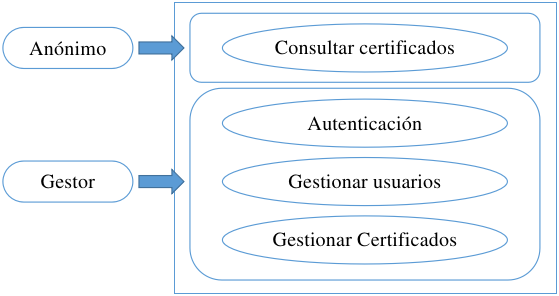
\includegraphics[width=\linewidth]{Graphics/caso-uso.png}
	\caption{Diagrama de casos de uso del sistema}
	\label{fig:11}
\end{figure}

En la Figura \ref{fig:11} se observa el diagrama de casos de uso del sistema a que se presenta. Los diagramas de casos de usos [\cite{91}] son un tipo de diagrama dónde se puede representar el comportamiento esperado del sistema, desde la visión de los usuarios, sin llegar a un alto nivel de especificación acerca de cómo se implementan las acciones. 

Los principales elementos que nos encontramos en él son:
\begin{itemize}
	\item Sistema: Representa con un rectángulo los límites del sistema, los actores se ubican fuera de la figura.
	\item Caso de uso: Representado con un óvalo y un texto identificativo, identifican una determinada acción.
	\item Actor: Son las entidades externas al sistema que interactúan con él.
\end{itemize}

Las acciones: gestionar certificados y gestionar usuarios se dividen a su vez un subacciones. Es necesario sobre estos modelos poder crear nuevas entradas y eliminar, editar o invalidar las existentes. En el caso de los certificados es necesario además un proceso de validación por tres usuarios gestores con roles específicos.

%\subsubsection{Descripción de los casos de uso del sistema}
En las tablas \ref{tab:CU1} y \ref{tab:CU2} se exponen dos de los casos de uso de alto nivel, para lograr entender los procesos globales de la aplicación. El resto puede ser encontrado en los anexos \ref{appendix:useCase}.

\begin{table}[!h]
	\begin{center}
		\begin{tabular}{|c|p{10cm}|}
			\hline \textbf{CU1} & Validar certificados \\ 
			\hline \textbf{Actor} & Gestor \\ 
			\hline \textbf{Descripción} & Ciertos usuarios de tipo gestor podrán validar los títulos asociados a una persona al introducir el identificador que representa al certificado.  \\ 
			\hline 
		\end{tabular}
		\caption{Caso de uso: Validar Certificado}
		\label{tab:CU1}
	\end{center}
\end{table}

\begin{table}[!h]
	\begin{center}
		\begin{tabular}{|c|p{10cm}|}
			\hline \textbf{CU2} & Autenticación \\ 
			\hline \textbf{Actor} & Gestor\\ 
			\hline \textbf{Descripción} & El usuario de tipo gestor deberá insertar sus credenciales (nombre de usuario y contraseña) para poder acceder al sistema.\\ 
			\hline 
		\end{tabular}
		\caption{Caso de uso: Autenticación}
		\label{tab:CU2}
	\end{center}
\end{table}

\subsection{Historias de usuario}
Las historias de usuario se usan, en el contexto de la ingeniería de requisitos ágil, como una herramienta de comunicación que combina las fortalezas de ambos medios: escrito y verbal. Describen, en una o dos frases, una funcionalidad de \textit{software} desde el punto de vista del usuario, con el lenguaje que éste emplearía. Se enfocan en qué necesidades o problemas soluciona lo que se va a construir.

Las tablas \ref{tab:HU1}, \ref{tab:HU2}, \ref{tab:HU3} se exponen algunos de las historias de uso de alto nivel, el resto pueden ser encontradas en los anexos \ref{appendix:useHistory}.

\begin{table}[!h]
	\begin{center}
		\begin{tabular}{|c|p{10cm}|}
			\hline \textbf{H.U-1} & Conocer títulos \\ 
			\hline \textbf{Usuario} & Anónimo\\ 
			\hline \textbf{Descripción} & Como usuario anónimo quiero poder conocer los certificados de una persona para poder observar las habilidades y estudios de esa persona. \\ 
			\hline 
		\end{tabular}
		\caption{Historia de Usuario: Conocer títulos}
		\label{tab:HU1}
	\end{center}
\end{table}

\begin{table}[!h]
	\begin{center}
		\begin{tabular}{|c|p{10cm}|}
			\hline \textbf{H.U-2} & Autentificación \\ 
			\hline \textbf{Usuario} & Gestor \\ 
			\hline \textbf{Descripción} & Como usuario gestor quiero poder autenticarme para poder tener acceso al sistema. \\ 
			\hline 
		\end{tabular}
		\caption{Historia de Usuario: Autentificación}
		\label{tab:HU2}
	\end{center}
\end{table}

\begin{table}[!h]
	\begin{center}
		\begin{tabular}{|c|p{10cm}|}
			\hline \textbf{H.U-3} & Cerrar sesión \\ 
			\hline \textbf{Usuario} & Gestor \\ 
			\hline \textbf{Descripción} & Como usuario gestor quiero poder cerrar la sesión actual para poder salir de forma segura del sistema. \\ 
			\hline 
		\end{tabular}
		\caption{Historia de Usuario: Cerrar sesión}
		\label{tab:HU3}
	\end{center}
\end{table}

%\subsection{Planificación de desarrollo}
%Siendo el equipo solamente una persona (el autor de este trabajo), no existe ningún rol, pero se mantiene la creación y el mantenimiento del \textit{backlog}, siguiendo una organización de \textit{sprints}, permitiendo tener alguna parte del sistema funcionando después de cada iteración, para que esto pudiera ser presentado y discutido con el cliente. Si el equipo aumentara en un futuro, se comenzaría a hacer uso de los roles definidos en la metodología.

%La fecha final del proyecto será acorde a la fecha límite de entrega de la convocatoria ordinaria del Trabajo de Fin de Grado. Por tanto, se ha establecido la duración de los sprints en 2 semanas, teniendo cada uno una carga de 34h aproximadamente por \textit{sprint}. En la tabla \ref{tab:sprints} puede verse una planificación inicial. Esta planificación es susceptible a cambios, así como la fecha de finalización podría ser cambiada.

%\begin{table}[!h]
	%\begin{center}
		%\begin{tabular}{|c|c|c|c|}
			%\hline \textbf{Sprint} & \textbf{Comienzo} & \textbf{Final} & \textbf{H.U a desarrollar} \\ 
			%\hline Sprint 0 & 3/09/2022  & 18/09/2022 & -\\ 
			%\hline Sprint 1 & 18/09/2022 & 2/09/2022 & H.U-1\\ 
			%\hline Sprint 2 & 2/09/2022 & 16/10/2022 & H.U-2, H.U-3\\ 
			%\hline Sprint 3 & 16/10/2022 & 30/10/2022 & H.U-4\\ 
			%\hline Sprint 4 & 30/10/2022 & 14/11/2022 & H.U-5, H.U-6, H.U-7\\ 
			%\hline Sprint 5 & 14/09/2022 & 25/10/2022 & H.U-8\\ 
			%\hline 
		%\end{tabular}
		%\caption{\textit{Backlog} inicial}
		%\label{tab:sprints}
	%\end{center}
%\end{table}

\section{Diseño del sistema}
En esta sección se describe cómo está ideado el sistema, pasando por su arquitectura, los patrones usados, los roles que tienen los usuarios y los datos que representan un certificado académico. Se puntualizarán también elementos de seguridad y será presentado el diagrama de despliegue del sistema.

\subsection{Arquitectura del sistema}
La arquitectura de un \textit{software} se encarga de entender cómo debe organizarse el sistema y cómo tiene que diseñarse la estructura global del mismo [\cite{91}]. Constituye el enlace crucial entre el diseño y la ingeniería de requisitos, ya que identifica los principales componentes estructurales en un sistema y la relación entre ellos. La salida del proceso de diseño arquitectónico consiste en un modelo arquitectónico que describe la  forma en que se organiza el sistema como un conjunto de componentes en comunicación. La arquitectura de \textit{software} representa un elemento fundamental pues afecta el desempeño del sistema, así como su capacidad de distribución y mantenimiento.

Según [\cite{99}], la arquitectura de un sistema puede basarse en un patrón o un estilo arquitectónico particular. Un patrón arquitectónico es una descripción de una organización del sistema, captan la esencia de una arquitectura usada en diferentes sistemas de \textit{software}.

Para este sistema se ha optado por dividirlo en dos niveles: lógica de negocio y persistencia (Figura \ref{fig:8}). 

\begin{figure}[h]
	\centering
	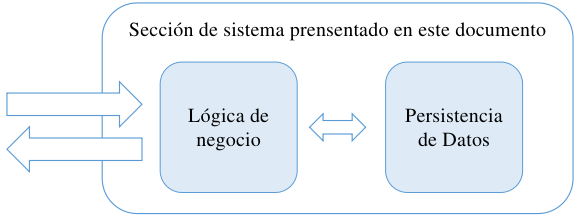
\includegraphics[width=\linewidth]{Graphics/arquitectura-bs.png}
	\caption{Arquitectura del sistema}
	\label{fig:8}
\end{figure}

El nivel de negocio es el encargado de facilitar al nivel de presentación los datos necesarios, a la vez que recolecta los datos aportados por este para procesarlos. Este nivel está conectado con el nivel de persistencia, enviándole peticiones para almacenar o recuperar datos de este [\cite{96}].

El nivel de persistencia es donde residen los datos y generalmente está formada por un gestor encargado de realizar el almacenamiento de datos. Este nivel recibe las peticiones de negocio, quien le dice qué datos necesita o qué datos tiene que almacenar [\cite{96}]. 

La persistencia de datos se divide en dos componentes: el almacenamiento de los usuarios y el de los certificados. Para almacenar los usuarios se escogió una base de datos relacional PostgreSQL, mientras que para almacenar los certificados se ha usado tecnología blockchain con el software Hyperledger Fabric. Ambas componentes son gestionadas por el nivel de negocio y entre ellas (Usuarios y Certificados) no tienen comunicación directa (Figura \ref{fig:9}).

\begin{figure}[h]
	\centering
	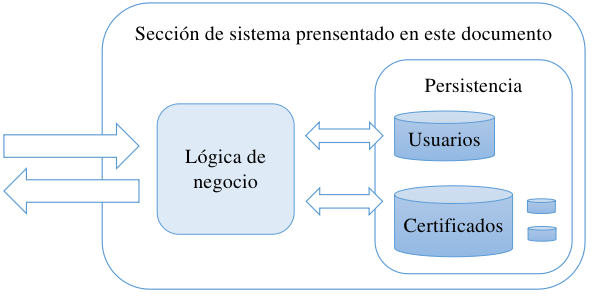
\includegraphics[width=\linewidth]{Graphics/arquitectura-ex.png}
	\caption{Arquitectura del sistema expandida}
	\label{fig:9}
\end{figure}

Durante el capítulo de Estado del Arte se explicó la razón de usar Go. Dado que esta capa lógica tiene que aceptar peticiones generadas por el nivel de presentación y marcar un límite bien definido entre ambas, se usa la biblioteca `Iris GO'. Iris Go es un web framework que permite crear los endpoints necesarios para un desacople limpio y poder afirmar que el sistema propuesto sigue una arquitectura cliente-servidor.

\subsection{Patrones de diseño seguidos}

La arquitectura es necesaria para comprender el sistema, organizar el desarrollo, fomentar la reutilización y hacer evolucionar el sistema. Para definirla es muy importante tener en cuenta un patrón de diseño o modelo de abstracción que nos sirva para poder estructurar de manera eficaz todos los componentes de la aplicación.

\subsubsection{Patrones GRASP}
Los patrones GRASP (Patrones Generales de Software para Asignación de Responsabilidades) describen los principios fundamentales de diseño de objetos para la asignación de responsabilidades. Las responsabilidades  están relacionadas con las obligaciones de un objeto en cuanto a su comportamiento [\cite{97}]. Entre los patrones GRASP empleados en la presente propuesta se encuentran:

\begin{itemize}
    \item Controlador: El patrón controlador es un patrón que sirve como intermediario entre una determinada interfaz y el algoritmo que la implementa. 

	Se dividen las distintas funcionalidades del sistema en endpoints que sean especializados y no genéricos. Cada uno de estos endpoints serán los encargados de utilizar los servicios que son los que saben como construir la respuesta. Con esta cantidad de endpoints se aumenta la cohesión y disminuye el acoplamiento.
	
	\item Bajo Acoplamiento: El acoplamiento es una medida de la fuerza con que una clase está conectada a otras clases, con que las conoce y recurre a ellas. El bajo acoplamiento soporta un diseño de clases más independientes, que reducen el impacto de cambios, y permite que sean más reutilizables.
	
	La capa de negocio implementada en go y basada en paquetes permite un bajo acoplamiento entre sus componentes. Estos pueden ser creados, modificados o eliminados en cualquier momento, lo que proporciona que la dependencia entre ellos sea baja.
	
	\item Alta Cohesión: La cohesión es una medida de la fuerza con la que se relacionan las clases y el grado de focalización de las responsabilidades de un elemento. Cada elemento del diseño debe realizar una labor única dentro del sistema, no desempeñada por el resto de los elementos, y auto-identificable. Una clase con baja cohesión realiza muchas labores no relacionadas o realiza demasiado trabajo.
	
	La capa de negocio implementada en go y basada en paquetes permite la organización del trabajo en cuanto a la estructura del proyecto y la asignación de responsabilidades con una alta cohesión. Cada componente realiza solo las funcionalidades para las cuales fueron creados, colaborando entre ellos para cumplir con el resto de las funcionalidades, generando un bajo acoplamiento y fomentando la reutilización. Esto hace posible que el sistema sea flexible a cambios sustanciales con efecto mínimo
\end{itemize}

\subsubsection{Patrones GoF}
Los patrones GoF(Gang of Four) utilizados en la propuesta de solución son los siguientes:

\begin{itemize}
	\item Bridge (Puente): Desacopla una abstracción de su implementación.
	
	El nivel de negocio tiene capas internas. Una de estas capas es la encargada de comunicarse con los framework que tratan la persistencia. De esta forma cuando un dato es requerido se le pide a esa capa, abstrayéndose de como es buscado. Esta capa sirve de puente entre ambos niveles: negocio y persistencia
	
	\item Command (Orden): Este patrón encapsula una operación en un objeto, permitiendo ejecutar dicha operación sin necesidad de conocer el contenido de la misma.
	
	El Proceso de validación de certificados sigue este patrón, Aún sin conocer el tipo de validador que sea
	el usuario este puede emitir la validación. El sistema se encargará luego de entender el proceso y modificar los campos pertinentes del certificado.	
\end{itemize}

\subsection{Roles de usuarios}

El proyecto consta con varios roles que tienen distintas funcionalidades. El personal de las instituciones universitarias podrán realizar consultas más especializadas y gestionar los certificados digitales según el rol que posea, para ello necesitarán iniciar sesión con sus credenciales asignadas. Los roles que se manejarán para los usuarios gestores son los siguientes:

\begin{itemize}
	\item \textbf{Administrador de Sistemas}: Encargado de manejar los usuarios que participan en el sistema: crearlos, editarlos, eliminarlos o invalidarle sus credenciales.
	\item \textbf{Administrador de Certificados}: Usuario que tiene los permisos para gestionar los certificados: crearlos, editarlos, eliminarlos o invalidarlos. Este rol no valida los certificados.
	\item \textbf{Secretario General}: Usuario que tiene los permisos para validar certificados recién creados. Puede invalidar los certificados que encuentre inconsistentes.
	\item \textbf{Decano de Facultad}: Usuario que tiene los permisos para validar certificados aprobados por el Secretario General. Puede invalidar los certificados que encuentre inconsistentes.
	\item \textbf{Rector de Universidad}: Usuario que tiene los permisos para validar certificados aprobados por el decano. Es el último eslabón para hacer un certificado válido. Puede invalidar los certificados que encuentre inconsistentes.
	\item \textbf{Inválido}: Usuario al que le fueron retirados sus privilegios por un administrador de sistema.
\end{itemize}

\subsection{Estructura de los certificados}
El sistema que se presenta no registrará binarios (copia digital de título, entre otras), sino que los certificados serán representados por propiedades:
\begin{itemize}
	\item \textbf{ID}: El identificador de los certificados es con fines de facilitar su búsqueda. No tiene una representación real en un certificado a papel. El campo es generado utilizando la fecha y hora de creación de la credencial. Su estructura es: YYYYMMDDHHMMSS (año, mes, día, hora, minuto y segundo concatenados)
	\item \textbf{Certificación}: Título que se le otorga al acreditado.
	\item \textbf{Título de oro}: Campo que representa si se alcanzó la distinción.
	\item \textbf{Emisor}: Centro que emite el certificado. Ej: Universidad de la Habana.
	\item \textbf{Acreditado}: Persona a la que se emite el título.
	\item \textbf{Fecha}: Fecha de emisión del documento.
	\item \textbf{Creador}: Usuario que creó dicho certificado en la base de datos.
	\item \textbf{Secretario, Decano y Rector}: Tres propiedades que guardan los nombres de los funcionarios que validan la Credencial.
	\item \textbf{Tomo y folio de facultad y universidad}: Dos propiedades que almacenan Tomo y folio bajo el cual fueron inscritos los documentos tanto en la facultad como en la universidad
	\item \textbf{Estado}: Refleja el estado actual del documento.
	\item \textbf{Razón de Invalidación}: Refleja, de estar el certificado en estado invalidado, la razón de la decisión.
\end{itemize}

Los certificados pueden tener cinco estados:
\begin{itemize}
	\item \textbf{Inválido}: El certificado fue invalidado por un usuario gestor con los permisos adecuados.
	\item \textbf{Creado}: El documento fue creado, pero no posee ninguna firma de validación.
	\item \textbf{Firmado por Secretario}: El documento fue validado por un usuario gestor con rol de `secretario'.
	\item \textbf{Firmado por Secretario y Decano}: El documento fue validado por un usuarios gestores con rol `secretario' y `decano'.
	\item \textbf{Válido}: El certificado fue validado por usuarios gestores con rol `secretario', `decano' y `rector'.
\end{itemize}

Los certificados tiene que pasar por varios estados en secuencia antes de tener el estado `Válido' [\ref{fig:12}]
\begin{figure}[h]
	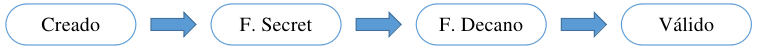
\includegraphics[width=\linewidth]{Graphics/status.png}
	\caption{Proceso de certificados hasta el estado de Válido}
	\label{fig:12}
\end{figure} 

\subsection{Elementos de seguridad}
La autenticación de portador (también llamada autenticación de token) es un esquema de autenticación HTTP que involucra tokens de seguridad llamados \textit{Bearer tokens} [\cite{98}]. El nombre ``Autenticación de portador'' puede entenderse como ``dar acceso al portador de este token''. El \textit{Bearer token} es una cadena críptica, generalmente generada por el servidor en respuesta a una solicitud de inicio de sesión. Este inicio de sesión es necesario para los gestores: actores del sistema que dependiendo de su rol tiene la capacidad de modificar los datos almacenados en la capa de persistencia. 
%Como habíamos mencionado previamente en la definición de actores del sistema, los gestores son usuarios registrados en un sistema de terceros y además cuentan con un rol definido en dicho sistema de terceros. Nuestra interfaz de usuario debe ser capaz de mostrar visualmente las secciones del \textit{back office} relacionadas a los permisos asociados al rol del usuario autenticado.

La solución propuesta en este trabajo creará y verificará tokens de identificación (\textit{Bearer token}) para cada usuario. Estos tokens serán entregados a la capa que se comunique con los endpoints, la cual enviará sus peticiones con estos tokens como muestra de la identidad. Codificado en estos está la información del nombre del usuario y su rol en el sistema. Cada endpoint, si así lo requiere, podrá consultar esos datos y controlar el acceso a esas funcionalidades.

Para evitar la autenticación de clientes mal intencionados que pretendan comprometer la seguridad de la base de datos donde se almacenan los usuarios; se guardará un hash de las contraseña en lugar de la contraseña misma. Como se sabe, por las cualidades de las funciones hash, conociendo el hash no se puede obtener la contraseña a partir de la cual se generó.

Para mantener la integridad de los datos almacenados en el nivel de persistencia se harán comprobaciones de validación. Estas comprobaciones serán realizadas si una operación que implique modificación de datos puede crear inconsistencia en estos. Un ejemplo del proceso está en la edición de certificados. El estado de un certificado representa los directivos que faltan por validarlo (o en casos particulares si está invalidado), una vez lleguen los nuevos valores de la edición se comprobará que en el certificado no falte ninguno de los validadores que su estado refleja ya han firmado.

\subsection{Diagrama de despliegue}
Un modelo de despliegue consiste en una representación estructural de la arquitectura del sistema desde el punto de vista de la distribución de los artefactos del software en los destinos de despliegue; definiendo a los artefactos como representaciones de elementos concretos en el mundo físico que son el resultado de un proceso de desarrollo [\cite{91}]. La Figura \ref{fig:10} representa el diagrama de despliegue del sistema que se propone.

\begin{figure}[h]
	\centering
	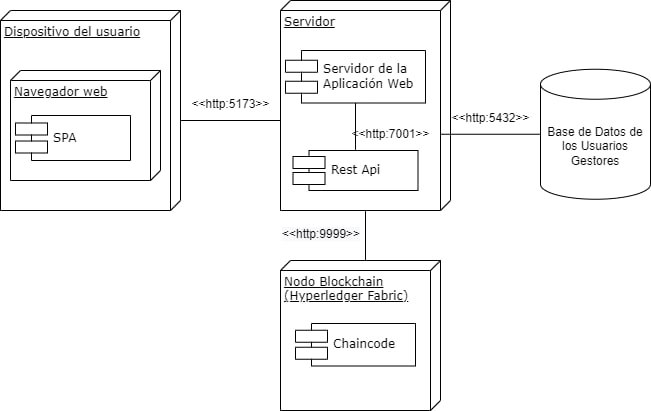
\includegraphics[width=\linewidth]{Graphics/diagrama.png}
	\caption{Diagrama de despliegue del sistema.}
	\label{fig:10}
\end{figure}


\chapter{Detalles de Implementación y Experimentos}\label{chapter:implementation}


\backmatter

\begin{conclusions}
    Conclusiones
\end{conclusions}

\begin{recomendations}
Una vez las autoridades pertinentes adopten y empiecen a aplicar el sistema se obtendría la retroalimentación necesaria para seguirlo mejorando. Se espera poder contar también con las opiniones de terceros desarrolladores interesados en conectarse a los endpoints del sistema.

Se recomienda en una futura versión conectar la dapp con una wallet para dotar de identidades criptográficas a los usuarios.
Otra opción podría ser usar una tecnología de identidad descentralizada como Hyperledger Indy. Teniendo los usuarios identidades criptográficas se logra una capa de seguridad extra. Por ejemplo, el proceso de validación de los certificados por el Secretario General, por el Decano de la facultad y por el Rector de la universidad podría realizarse usando el concepto de llave pública y privada de la criptografía asimétrica.

Se aconseja también utilizar Casbin como biblioteca que maneja el control de acceso a funcionalidades. Casbin permite abordar la problemática de una manera escalable y elegante.

Por otro lado se recomienda utilizar los conocimientos de los modelos relacionales y reestructurar los datos de los Certificados. Si se lleva su representación a una estructura que cumpla con la Tercera Forma Normal se logrará ahorrar espacio y eliminar potenciales multirepresentaciones del mismo dato.

La infraestructura aquí descrita puede ser aprovechada para más que los títulos, pueden incluirse también certificaciones de notas, planes de estudios o acreditaciones de publicaciones de artículos y libros. El sistema aquí propuesto puede convertirse en la traza de todo el recorrido educacional e investigativo de los egresados con nivel de estudios superiores en Cuba. Siendo tan sencillo conocer las credenciales de una persona como dar un click.
\end{recomendations}

\printbibliography[heading=bibintoc]


\end{document}